\chapter{Introduction to Computational Complexity}
\lecture{16}{8 Nov. 17:00}{}

\section{Introduction}
\textbf{Computational complexity}는 computational problem을 풀기 위해서 필요로하는 자원의 종류인 time, space의 요구량을 분석하는 연구이다.
Computational complexity의 주요 연구는 어떤 문제를 풀기 위한 best algorithm이 요구하는 자원의 양이 input size에 대해 어떤 lower bound를 가지는 것을 증명하는 것이다. 이는 심지어 그 문제를 해결하는 알고리즘이 구체적으로 무엇인지 알지 못하더라도 논의될 수 있다.

\textit{Strong Church-Turing thesis}는 모든 computational model이 probabilistic Turing machine에서 Polynomial time으로 시뮬레이션 할 수 있다고 주장한다. 양자 컴퓨터가 주목받고 있는 이유 중 하나로는 양자 컴퓨터가 classical computer가 polynomial time에 효과적으로 해결할 수 없으리라고 여겨졌던 문제들을 효과적으로 해결하는 경우가 발생하고 있기 때문이다. 이러한 결과들은 Strong Church-Turing thesis에 대해 의문을 제기하게 만든다.

Computational complexity를 다룸에 있어서 주의해야할 사항은 어떤 문제를 해결하는데 exponential resource가 요구된다는 것을 "엄밀하게" 증명하는 것은 매우 까다롭다는 사실이다. (e.g., NP problem)
이는 quantum computer에 대해서도 중요한 문제 중 하나인데 만약 양자컴퓨터가 polynomial time에 해결할 수 있는 NP problem이 사실은 P class에 속한다는 것이 증명된다면 quantum computer로서 얻을 수 있는 계산적 이점이 사라지기 떄문이다.

\section{The class NP: Reducibility and completeness}
\subsection{P and NP problems}
우리는 지금부터 computational complexity를 다루기 위해 "YES / NO"라는 답변을 하는 \textit{decision problem}에 대해서만 집중하고자 한다. Output이 2가지라는 측면에서, 이러한 problem은 output이 one-bit은 boolean function $f: \{0, 1\}^* \rightarrow \{0, 1\}$로 나타낼 수 있다.

Turing machine이 어떤 language $L \subset \{0, 1\}^*$에 속하는 모든 word를 \textit{decide}할 수 있을 떄, 그 machine이 함수 $f_L : \{0, 1\}^* \rightarrow \{0, 1\},\quad f_L(x) = 1 \Leftrightarrow x \in L$를 계산한다고 한다.
\begin{definition}\label{def:P-class}
    모든 $x \in \{0, 1\}^*$에 대해 polynomial time에 $f_L$을 계산할 수 있는 turing machine $M$이 존재한다면, language $L \subset \{0, 1\}^*$이 P class에 속한다고 한다.
    \begin{equation*}
        x \in L \Longleftrightarrow M(x)=1, \quad x \notin L \Longleftrightarrow M(x)=0 .
    \end{equation*}
\end{definition}

P는 직접적으로 주어진 문제를 해결하는 것과 관련 있다. 그러나 어떤 경우에는, 직접 문제를 푸는 것보다 적절한 \textit{hint}가 주어졌을 때 해답을 검증하는 것이 더 효율적일 수 있다.\footnote{efficiently verifiable solutions} 

"효율적으로 검증 가능한 문제"를 엄밀하게 다루기 위해서 먼저 NP class를 정의하자.
\begin{definition}\label{def:NP-class}
    모든 $x \in \{0, 1\}^*$에 대해 다음을 만족하는 polynomial time TM $M$과 polynomial $p: \mathbb N \rightarrow \mathbb N$가 존재한다면, language $L \subset \{0, 1\}^*$이 NP class에 속한다고 한다.
    $$ \begin{aligned}
        & x \in L \Longleftrightarrow \exists u \in\{0,1\}^{p(|x|)} \text { s.t. } M(x, u)=1 \\
        & x \notin L \Longleftrightarrow \forall u \in\{0,1\}^{p(|x|)} \text { s.t. } M(x, u)=0
    \end{aligned} $$
    $x \in L $에 대해 $M(x, u)=1$가 되게하는 $u \in\{0,1\}^{p(|x|)}$를\footnote{i.e., $M$이 polynomial time에 $x$가 solution인지 아닌지를 확인할 수 있게 만드는 hint $u$} $x$에 대한 \textit{certificate(or witness)}라고 부른다.
\end{definition}

여기서 한 가지 주목할 점은 NP를 정의할 때, 그 문제를 풀기 위해서 요구되는 자원의 양이 얼마나 많이 필요한지는 정의하지 않았다는 점이다. NP는 단지 효율적으로 검증할 수 있는 문제들의 집합이다.

\vspace{1em}

다음은 NP의 정의를 만족하는 decision problem의 예시들이다.
\begin{itemize}
    \item Independent set problem: 그래프 $G$와 $k$가 주어졌을 떄, $k$-size의 independent set이 존재하는지 확인하는 문제. $\rightarrow$ (\textit{witness}) independent set이 존재한다면, 그 set의 원소들을 제공한다.
    \item Traveling salesman problem: 그래프 $G$와 각 edge의 가중치가 주어졌을 떄, 가중치의 합이 $k$를 넘지 않으며 모든 노드를 정확히 한번씩만 방문하는 closed path가 존재하는지 확인하는 문제. $\rightarrow$ (\textit{witness}) 최단 경로가 존재한다면, 그 경로를 제공한다.
    \item Subset sum problem: $n$개의 정수 $A_1, \cdots, A_n$과 정수 $T$가 주어졌을 떄, 원소들의 합이 $T$가 되는 subset이 존재하는지 확인하는 문제. $\rightarrow$ (\textit{witness}) subset이 존재한다면, 그 subset의 원소들을 제공한다.
\end{itemize}

\vspace{1em}

이렇게 P, NP를 정의하면 각 complexity class간의 관계를 생각해볼 수 있다.
\begin{itemize}
    \item $P \subset NP$\footnote{$P\subset NP$인지, $P\subseteq NP$인지는 아직 밝혀지지 않았다.} : 만약 $L \in P$가 TM $N$을 사용하여 poly-time에 decide될 때, TM $N$을 zero-polynomial witness $p(x)$ (i.e., empty)와 함께 사용하여 $x$를 poly-time에 decide할 수 있으므로 $L \in NP$이다.
    \item $NP \subset EXP$ : 만약 $L \in NP$가 TM $M$, witness $p()$를 사용하여 poly-time에 decide될 때, TM $M$을 사용하여 모든 가능한 witness를 대입해보면서 $x$가 solution인지 아닌지 decide할 수 있으므로 $L \in EXP$이다. ($2^{O(p(n))} \approx O(2^{n^c})$ time\footnote{ Since $O(p(n)) = O(n^c)$ for some constant c})
\end{itemize}

Nondeterministic turing machine을 이용하면, NP를 다르게 정의할 수도 있다. NDTM은 매 step마다 2가지 서로 다른 transition function $\delta_0$, $\delta_1$중에서 하나를 선택할 수 있다. 모든 $x$에 대해 accept state에 도달하게 만드는 선택의 조합이 존재할 때, $M(x) = 1$이며 그렇지 않을 경우 $M(x) = 0$이다. NDTM에서의 witness는 이러한 선택의 조합을 제공하는 것이다.
\begin{definition}\label{def:NP-alt}
    모든 $x \in \{0, 1\}^*$에 대해 다음을 만족하는 polynomial time NDTM $M$과 polynomial $p: \mathbb N \rightarrow \mathbb N$가 존재한다면, language $L \subset \{0, 1\}^*$이 $NP$ class에 속한다고 한다.
    $$ \begin{aligned}
        & x \in L \Longleftrightarrow M(x)=1 \\
        & x \notin L \Longleftrightarrow M(x)=0 .
    \end{aligned} $$
\end{definition}

\subsection{Reducibility and NP-completeness}
특정 class에 속하는 문제들중에서 \textbf{가장 어려운 문제}는 어떻게 정의할 수 있을까? Computational complexity에서는 이를 위해 \textit{reduction}을 사용한다.
\begin{definition}\label{def:reduction}
    다음을 만족하는 polynomial time computable function $f: \{0, 1\}^* \rightarrow \{0, 1\}^*$가 존재한다면, language $L \subset \{0, 1\}^*$이 $L' \subset \{0, 1\}^*$에 \textit{polynomial time reducible}이라고 한다.
    \begin{equation*}
        \forall x \in \{0, 1\}^*, \quad x \in L \quad if \ and \ only\ if \quad  f(x) \in L' .
    \end{equation*}
\end{definition}

직관적으로, reduction을 이용한다면 language $L$에 속하는 word $x$를 decide하는 대신, poly-time에 $f(x)$를 계산하여 language $L'$에 속하는 $f(x)$를 decide하는 문제로 바꿔서 생각할 수 있다. 따라서 $L$의 complexity는 $L'$의 complexity보다 복잡할 수 없다. \footnote{$L$을 푸는문제를 $L'$을 푸는문제로 바꾸는데 걸리는 복잡도가 polynomial이므로}

\begin{definition}\label{def:NP-complete}
    NP에 속하는 어떤 문제도 $L'$로 polynomial time reduction될 때, $L'$을 \textit{NP-hard}라고 하며, NP-hard이면서 동시에 NP에 속하는 문제를 \textit{NP-complete}이라고 한다.\footnote{$\text{NP-complete} = \text{NP-hard} \cap \text{NP}$}
\end{definition}

\begin{figure}[h]
    \centering
    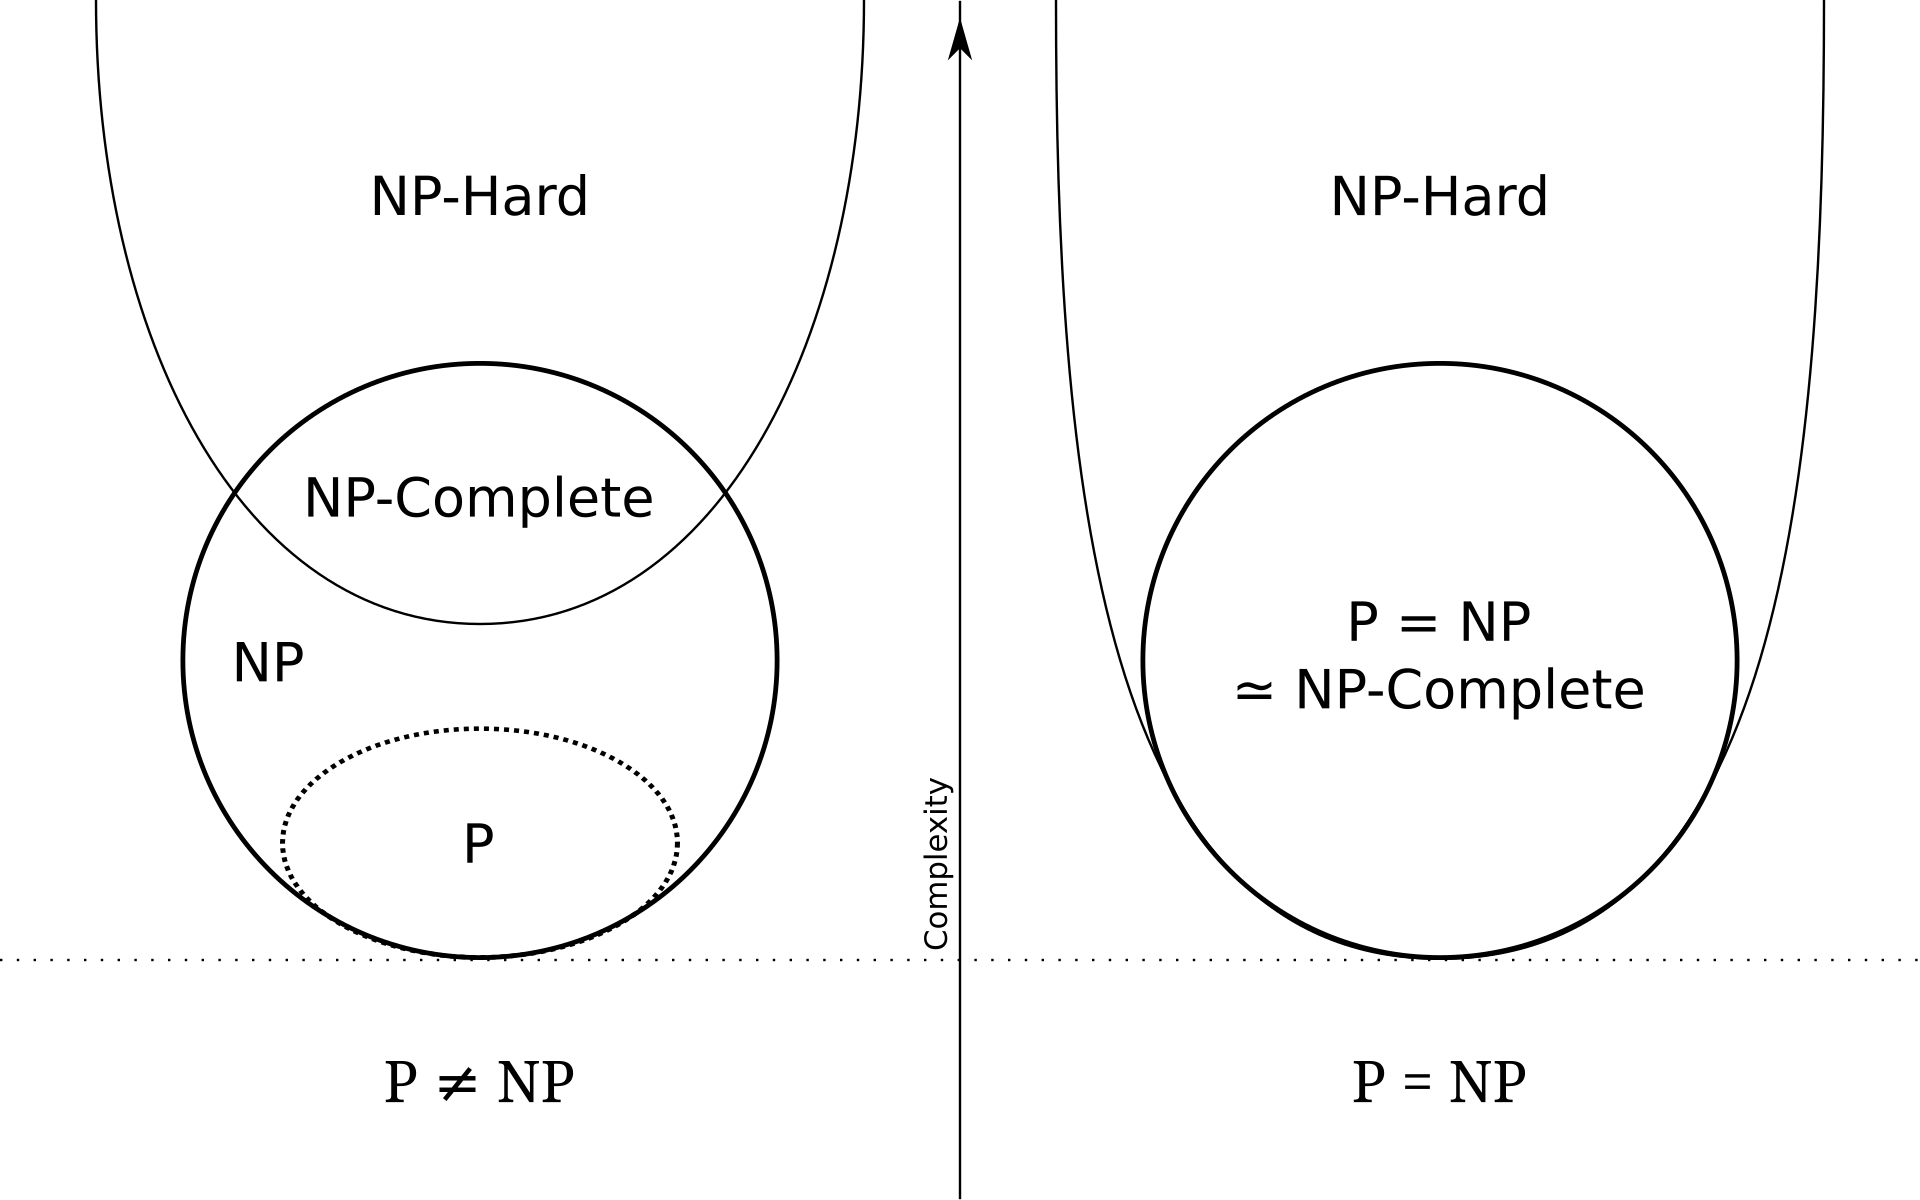
\includegraphics[width=0.48\textwidth]{figures/P_np_np-complete_np-hard.png}
    \caption{P and NP class \cite{NP-wiki}}
    \label{fig:NP-class}
\end{figure}

\lecture{17}{11 Nov. 17:00}{}
\subsection{Boolean formula and Cook-Levin theorem}
앞에서 우리는 NP에 속하는 여러 문제들의 예시를 살펴보았다. 이제 NP-complete에 속하는 문제 \textit{3-SAT problem}를 소개하려고한다. 이를 위해서 먼저 boolean formula에 대해 알아보자.

Boolean formula는 boolean variable $u_1, \cdots, u_n$과 logical operator NOT($\neg$), OR($\vee$), AND($\wedge$)로 구성되는 수식이다. 어떤 boolean formula를 나타내는 변수를 $\varphi$라고 정의할 때, boolean formula를 이루는 각각의 변수에 어떤 값을 대입하였는지를 $z \in \{0, 1\}^n$으로 표현하자. 이때, $\varphi(z) = 1$이 되도록하는 $z$가 존재한다면 $\varphi$는 \textit{satisfiable}이다. (e.g., $\varphi = u_1 \vee \neg u_2$ is satisfiable for $z = (1, 0)$)
\\특히 어떤 boolean formula가 \textit{conjunctive normal form}이라는 의미는 변수들의 OR의 AND로 이루어진 수식이라는 의미이다. 예를 들어,
\begin{equation*}
    \left(u_1 \vee \bar{u}_2 \vee u_3\right) \wedge\left(u_2 \vee \bar{u}_3 \vee u_4\right) \wedge\left(\bar{u}_1 \vee u_3 \vee \bar{u}_4\right),
\end{equation*}
또는 일반화하여 나타내면 다음과 같다.
\begin{equation*}
    \bigwedge_i\Big(\bigvee_j v_{i_j}\Big)
\end{equation*}
이제 우리는 language SAT을 다음과 같이 정의할 수 있다.
\begin{definition}\label{def:SAT}
    Language \textbf{SAT}은 모든 가능한 satisfiable CNF formula들의 집합이다.\footnote{변수가 3개인 satisfiable CNF formula들의 집합을 3-SAT이라고 한다.} 즉, SAT problem은 주어진 boolean formula $x$가 satisfiable한지 결정하는 문제이다. 
\end{definition}

\begin{theorem}[Cook-Levin theorem]\label{thm:Cook-Levin}
    1. SAT is NP-complete, and 2. 3-SAT is NP-complete.
\end{theorem}
만약 주어진 boolean formula가 satisfiable하다면, $\varphi(z) = 1$이 되도록하는 $z$를 witness로 제공하면 문제를 풀 수 있기 때문에 SAT이 NP에 속한다는 것은 쉽게 증명할 수 있다. NP-hard에 속한다는 것을 증명하기 위해 NP에 속하는 모든 문제가 SAT로 reduction될 수 있음을 증명하면 된다.

이 수업에서는 SAT로의 reduction을 이용하는 대표적인 문제인 \textit{Classical Hamiltonian problem}에 대해서 살펴보고자 한다. 다음과 같은 3-local Hamiltonian을 가정하자.
\begin{equation*}
    H=\sum_{c=1}^m H_c\left(x_{c_1}, x_{c_2}, x_{c_3}\right)
\end{equation*}
Hamiltonian problem은 ground state의 energy를 계산하는 문제이므로 다음과 같이 표현할 수 있다.
\begin{equation*}
    H_c\left(x_{c_1}, x_{c_2}, x_{c_3}\right)=0,\qquad x \in \{-1, 1\}
\end{equation*}
즉, boolean function의 값이 $1$이 되도록하는 3-SAT problem과 유사한 형태를 보이는 것을 알 수 있다. 
\begin{equation*}
    f_c\left(u_{c_1}, u_{c_2}, u_{c_3}\right) = u_{c_1} \vee \bar{u}_{c_2} \vee u_{c_3} = 1,\qquad u \in \{0, 1\}
\end{equation*}
이를 이용하면, SAT problem의 결과로부터 Hamiltonian problem의 결과를 쉽게 계산할 수 있다. 다음과 같이 Hamiltonian을 계산하면, $f_c = 1$이 되도록하는 조합에 대해, Hamiltonian의 energy가 0이 되는 것을 알 수 있다. (e.g., $(1, 0, 0)$ for $f_c = 1$, then $H_c = 0$.)
\begin{equation*}
    \frac{1-u_{c_1}}{2} \frac{1+u_{c_2}}{2} \frac{1-u_{c_3}}{2}
\end{equation*}

\section{Quantum complexity}
\subsection{Probabilistic algorithms}
Quantum computer의 complexity를 정의하기 전에 먼저, 우리에게 익숙한 deterministic algorithm에서 벗어나 \textit{probabilistic algorithm}에 대해 살펴보자. Probabilistic algorithm을 수행하는 \textit{probabilistic Turing machine}은 NDTM처럼 2개의 서로 다른 transition function $\delta_0$, $\delta_1$을 가지며, 각각의 step마다 두 함수 중 하나를 $1/2$의 확률로 선택하여 수행한다. 확률에 따라서 동작하기 때문에 $x \in L$이 input으로 주어지더라도 TM이 종료되었을 때 reject state에 도달하게 되면 reject이라고 답한다.
\begin{definition}\label{def:BPP}
    모든 $x \in \{0, 1\}^*$에 대해 다음을 만족하는 polynomial time PTM $M$이 존재한다면, language $L \subset \{0, 1\}^*$이 $BPP$\footnote{bounded-error probabilistic polynomial} class에 속한다고 한다.\footnote{$M(x)$의 결과가 틀리지 않을 확률이 2/3이상}
    \begin{equation*}
        \operatorname{Pr}[M(x)=L(x)] \geq \frac{2}{3}
    \end{equation*}
\end{definition}
\begin{definition}\label{def:BPP-alt}
    모든 $x \in \{0, 1\}^*$에 대해 다음을 만족하는 polynomial time TM $M$과 polynomial $p: \mathbb N \rightarrow \mathbb N$가 존재한다면, language $L \subset \{0, 1\}^*$이 $BPP$ class에 속한다고 한다.\footnote{이때 $r$은 TM $M$에 random하게 추가되는 random bits.}
    \begin{equation*}
        \operatorname{Pr}_{r \in \{0, 1\}^{p(|x|)}}[M(x, r)=L(x)] \geq \frac{2}{3}
    \end{equation*}
\end{definition}
PTM에 대한 NP problem은 다음과 같이 정의된다.
\begin{definition}\label{def:MA}
    모든 $x \in \{0, 1\}^*$에 대해 다음을 만족하는 polynomial time TM $M$과 polynomial $p: \mathbb N \rightarrow \mathbb N$가 존재한다면, language $L \subset \{0, 1\}^*$이 $MA$\footnote{Merlin-Arthur} class에 속한다고 한다.
    $$ 
    \begin{aligned}
        & x \in L \Longleftrightarrow \exists u \in\{0,1\}^{p(|x|)} \text { s.t. } \operatorname{Pr}_r[M(x, u, r)=1] \geq \frac{2}{3} \\
        & x \notin L \Longleftrightarrow \forall u \in\{0,1\}^{p(|x|)} \text { s.t. } \operatorname{Pr}_r[M(x, u, r)=0] \geq \frac{2}{3} .
    \end{aligned}
    $$
\end{definition}
\vspace{-0.5em}
\subsection{Quantum algorithms}
이제 PTM에 대한 complexity class를 확장하여 Quantum computer에 대한 class를 정의해보자.
\begin{definition}\label{def:BQP}
    모든 $x \in \{0, 1\}^*$에 대해 다음을 만족하는  uniform family of polynomial time quantum circuits $\{Q_n : n \in \mathbb N\}$가 존재한다면, language $L \subset \{0, 1\}^*$이 $BQP$\footnote{bounded-error quantum polynomial} class에 속한다고 한다.
    $$ \operatorname{Pr}\left[Q_{|x|}(x)=L(x)\right] \geq \frac{2}{3} $$
\end{definition}

BQP class는 Quantum circuit으로 문제를 풀었을 때, 오류가 발생할 확률이 1/3 이하인 문제들의 집합이다. BQP class에 속하면서 P class에 속하지 않을 것이라고 믿는 문제들이 바로 quantum algorithm으로 해결하기 효과적인 문제들이다. (e.g., prime factorization) $Q(x)$를 실행한 뒤 첫 번쨰 qubit을 측정하여 그 값이 0인지 1인지를 기준으로 decidable problem을 해결할 수 있다.

\begin{definition}\label{def:QMA}
    모든 $x \in \{0, 1\}^*$에 대해 다음을 만족하는  uniform family of polynomial time quantum circuits $\{Q_n : n \in \mathbb N\}$과 quantum state\footnote{classical algorithm의 hint 역할}$\ket \psi$이 존재한다면, language $L \subset \{0, 1\}^*$이 $QMA$ class에 속한다고 한다.
    $$ \operatorname{Pr}\left[Q_{|x|}(x,|\psi\rangle)=L(x)\right] \geq \frac{2}{3} $$
\end{definition}

QMA에 속하는 대표적인 예시로 \textit{k-local Hamiltonian problem}이 있다. 다음과 같이 주어진 $k$-local Hamiltonian이 있을 때,
\begin{equation*}
    H = \sum^L_{i=1} H_i, \qquad (\|H_i\|_1 \le 1)
\end{equation*}
Hamiltonian의 ground state energy가 특정한 threshold $b$ 이상인지, 또는 $a$ 이하인지를 결정하는 문제이다. ($b-a=\Omega\left(n^{-\alpha}\right)$) $k$-local Hamiltonian problem이 QMA에 속하는 이유는, phase estimation algorithm을 이용하여 eigen-value를 추정하고 그 값이 $b \ge$, $a \le$인지를 확인하는 것으로 문제를 해결할 수 있기 때문이다.

더 나아가, $k$-local Hamiltonian problem은 QMA-complete이기 때문에 SAT problem처럼 QMA에 속하는 모든 문제들은 $k$-local Hamiltonian problem으로 reduction 될 수 있다.
\vspace{-0.5em}
\subsection{BQP vs PSPACE}
마지막으로, BQP class와 PSPACE class의 관계를 살펴보면서 complexity class간의 관계를 정리해보자.
\begin{definition}\label{def:PSPACE}
    TM이 input size에 대해 polynomial space와 arbitrary time을 사용하여 문제를 해결할 수 있을 때, language $L \subset \{0, 1\}^*$이 $PSPACE$ class에 속한다고 한다.
\end{definition}
BQP $\ne$ PSPACE에 대해서는 아직 모르지만, BQP $\subset$ PSPACE 관계에 대해서는 증명할 수 있다.

$U= U_T \cdots U_1$인 unitary gate를 가정하자. ($T = \text{poly}(n)$)\footnote{$T$가 input qubit에 대해 polynomial이므로, 이 gate $U$는 BQP에 속한다.} 이때 각 gate는 $\{C(X)$, single-qubit gate$\}$중 하나이며, 따라서 각 gate는 최대 2개의 qubit에만 작용할 수 있다.
Input qubit $n$개에 추가로 중간 계산을 위해 ancilla qubit $n$개를 사용한다고 가정하자. 그러면 $U$를 적용한 뒤, 첫 번째 qubit을 관측했을 때 그 결과가 0이 될 확률은 amplitude를 계산해서 얻을 수 있다. ($\ket{\mathbf y} = \ket 0 \ket{\mathbf y'}$)
\begin{equation*}
    \langle\boldsymbol{y}| U_T \cdots U_1\left|x^n, 0^n\right\rangle=\sum_{x_1, \ldots, x_{T-1} \in\{0,1\}^n}\langle\boldsymbol{y}| U_T\left|x_{T-1}\right\rangle \cdots\left\langle x_2\right| U_2\left|x_1\right\rangle\left\langle x_1\right| U_1\left|x^n, 0^n\right\rangle .
\end{equation*}
이 때, $\Sigma$를 이루는 각각의 term을 계산하기 위해서 필요한 space는 poly-space이므로 확률을 구하는 문제는 PSPACE에 속한다. 따라서 $BQP \subset PSPACE$이다.$\Box$
\begin{note}[Summary] $P \subset BPP \subset BQP \subset PSPACE$
\end{note}
\begin{figure}[h]
    \centering
    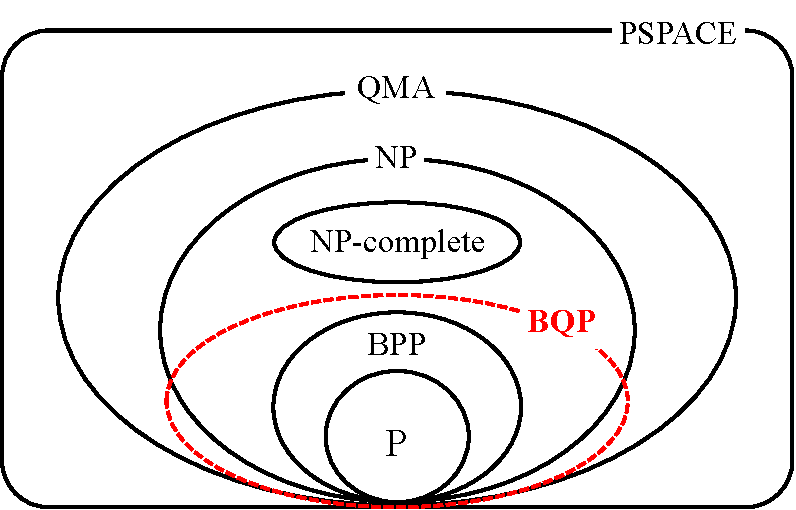
\includegraphics[width=0.43\textwidth]{figures/class.pdf}
    \caption{Computational complexity class}
    \label{fig:BQP-PSPACE}
\end{figure}